\subsection{Strong Interactions}
\label{sec:Intro_QCD}

\begin{figure}[htb]
  \begin{center}
    {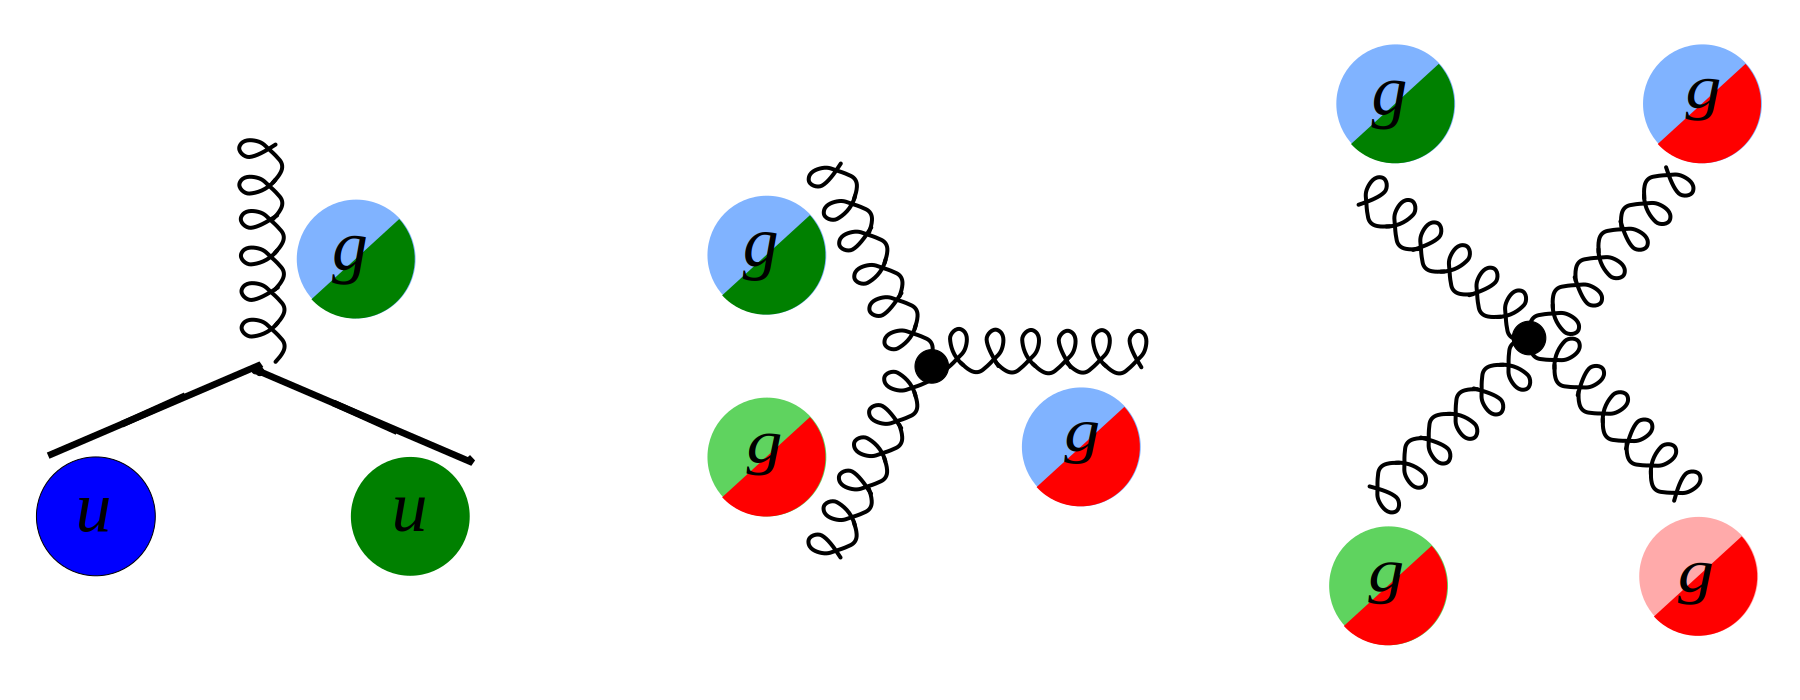
\includegraphics[width=0.90\textwidth]{../figs/Intro/feynmStrong.png}}
    \caption{Strong interations}
    \label{fig:feynmStrong}
  \end{center}
\end{figure}

The strong interactions are performed by exchanging a gluon. Only particles which possess a color charge can participate in the strong interactions (quarks, antiquarks, and gluons). There are eight types of gluons corresponding to different color-anticolor combinations. Gluons are spin-one massless electrically neutral particles. Gluons possess color charges, therefore, they can self-interact. 

The elementary strong processes are shown in Fig. \ref{fig:feynmStrong}. There are three elementary processes: qqg, ggg and gggg. Both electrical and color charges must be conserved at each vertex.

The coupling constant of the strong interaction depends on a distance between interacting particles: it becomes larger as the distance becomes smaller. This property leads to two consequences: the confinement and the asymptotic freedom.

The confinement comes from the fact that the interaction at large distances becomes stronger. That makes quarks always stay in the colorless combinations (hadrons). A combination becomes colorless when there is the same amount of color and anticolor or if there is the same amount of each of the three colors.  Mesons are comprised of a quark and antiquarks with the opposite color charges. The baryons are comprised of three quarks: a red, a green and a blue one.

The asymptotic freedom means that when quarks are very close to each other they almost do not interact with each other and therefore they are free. 

When the distance between quarks is low which corresponds to high energy, and thus the coupling constant $1/\alpha_s \ll 1$ is low, the strong interactions can be described by a perturbative theory which is called quantum chromodynamics (QCD). When the coupling constant is large, it is not possible to use a perturbative theory. 
